%\documentclass{beamer}
%\documentclass[c]{beamer}
 \documentclass[t]{beamer}
%\documentclass[b]{beamer}
\listfiles

\mode<presentation>
{
% \usetheme[english]{KIT}
% \usetheme[usefoot]{KIT}
  \usetheme[deutsch]{KIT}

%%  \usefonttheme{structurebold}

  \setbeamercovered{transparent}

  %\setbeamertemplate{enumerate items}[circle]
  \setbeamertemplate{enumerate items}[ball]
}

\usepackage{babel}
\date{10.05.2010}
%\DateText

%\KITfoot{\parbox[t]{90mm}{\today:\qquad Dies ist eine sehr lange selbstdefinierte Fu\ss{}zeile -- Dies ist eine sehr lange selbstdefinierte Fu\ss{}zeile -- Dies ist eine sehr lange selbstdefinierte Fu\ss{}zeile}}


\usepackage[latin1]{inputenc}
\usepackage[TS1,T1]{fontenc}
\usepackage{array}
\usepackage{lipsum}

\usenavigationsymbols
%\usenavigationsymbols[sfHhdb]
%\usenavigationsymbols[sfhHb]

\title[Beispiel eines ganz besonders langen Titels in der Fu�zeile, der zu lang f�r die Zeile ist und daher umgebrochen werden muss]{Beispiel einer Titelzeile}
\subtitle{Beispiel f�r einen Untertitel}

\author{KIT}

\institute{INSTITUTS- FAKULT�TS-, ABTEILUNGSNAME}

\TitleImage[height=\titleimageht]{Bilder/bildwand.jpg}

\newcommand{\itemsiii}{
  \item Uter res comprovincialis placitum opus alo Liceo, ploro an at lenocinium.
        Iuste Immanitas dux sus conclamo an Diuturnus
  \item Fatigo, almus ut erro cupido res famulatus Adstringo
  \item Stupendum commemoro Annuo ars quies Polliceor
}
\newcommand{\itemsi}{
  \item Ne necne Ne ymo iam Vota, Rutilus dux scelus internuntius.
}


\newcommand{\parxmpl}{
  Uter res comprovincialis placitum opus alo Liceo, ploro an at lenocinium.
  Iuste Immanitas dux sus conclamo an Diuturnus
  Fatigo, almus ut erro cupido res famulatus Adstringo
  Stupendum commemoro Annuo ars quies Polliceor
}
\newcommand{\Parxmpl}{
  Iuste Immanitas dux sus conclamo an Diuturnus
  Fatigo, almus ut erro cupido res famulatus Adstringo
}

\begin{document}

\begin{frame}
  \maketitle
\end{frame}

\begin{frame}
 \frametitle{Folientitel\\zweizeilig}

  \heading{Zwischen�berschrift}
  \begin{itemize}
  \itemsiii
  \end{itemize}
  \bigskip

  \heading{Zwischen�berschrift}
  \begin{itemize}
  \itemsiii
  \end{itemize}
  \vfill
  \mbox{}
\end{frame}

\begin{frame}
  \frametitle{Bild und Text 1}

  \begin{columns}[T]
    \column{57mm}
    \begin{itemize}\small
    \itemsi
    \itemsiii
    \end{itemize}
    \column{50mm}
    \hspace*{-6mm}\hfill
\includegraphics[width=54mm]{Bilder/tasten.jpg}
  \end{columns}
\end{frame}

\begin{frame}
  \frametitle{Bild und Text 2}
  \framesubtitle{Ein Bild am Anfang}

  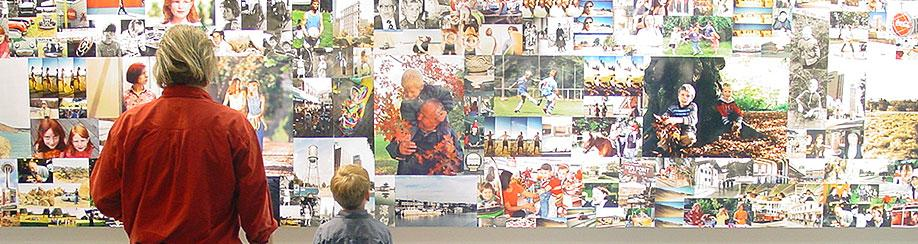
\includegraphics[width=\textwidth]{Bilder/bildwand.jpg}

  \begin{itemize}\small
  \itemsi
  \itemsiii
  \end{itemize}
  \vfill
  \mbox{}
\end{frame}

\begin{frame}
  \frametitle{Aufz�hlung}
  \framesubtitle{Mit Zwischen�berschriften}

  \heading{Zwischen�berschrift}
  \begin{itemize}
  \itemsiii
  \end{itemize}
  \bigskip

  \heading{Zwischen�berschrift}
  \begin{enumerate}
  \itemsiii
  \end{enumerate}
  \vfill
  \mbox{}
\end{frame}

\begin{frame}
  \frametitle{Das KIT-Logo}

  \KITimage[width=.3\textwidth]{Bilder/tasten}
  \hfill
  \KITframe{\parbox{4cm}{%
    \begin{itemize}
    \item Eins
    \item Zwei
    \item Drei
    \end{itemize}}}
  \bigskip

  \setlength{\vgdist}{.01\textwidth}
  \KITvectorgraphics[width=.3\textwidth]{Bilder/Small}
  \qquad
  \KITframe[bg]{\parbox{4cm}{%
    \begin{itemize}
      \item Eins
      \item Zwei
      \item Drei
    \end{itemize}}}
\end{frame}

\begin{frame}
  \frametitle{Mathematische Formeln}

  Mathematische Formeln werden mit dem Paket mathpazo gesetzt.

  \[a = \sqrt{b} + c^2 + \sum_{i=1}^\infty a_i\]
\end{frame}

\begin{frame}
  \frametitle{Fontgr��en}

  Die folgenden Fontgr��en sind vorgesehen:

  \begin{tabular}{>{\ttfamily}ll}
  \textbackslash tiny & \tiny tiny \quad \(x=\sqrt{2}, y=2^{2^2}\) \\
  \textbackslash scriptsize & \scriptsize scriptsize \quad \(x=\sqrt{2}, y=2^{2^2}\) \\
  \textbackslash footnotesize & \footnotesize footnotesize \quad \(x=\sqrt{2}, y=2^{2^2}\) \\
  \textbackslash small & \small small \quad \(x=\sqrt{2}, y=2^{2^2}\) \\
  \textbackslash normalsize & \normalsize normalsize \quad \(x=\sqrt{2}, y=2^{2^2}\) \\
  \textbackslash large & \large large \quad \(x=\sqrt{2}, y=2^{2^2}\) \\
  \textbackslash Large & \Large Large \quad \(x=\sqrt{2}, y=2^{2^2}\) \\
  \textbackslash LARGE & \LARGE LARGE \quad \(x=\sqrt{2}, y=2^{2^2}\) \\
  \textbackslash huge & \huge huge \quad \(x=\sqrt{2}, y=2^{2^2}\) \\
  \textbackslash Huge & \Huge Huge \quad \(x=\sqrt{2}, y=2^{2^2}\)
  \end{tabular}
\end{frame}

\setlength{\parskip}{.6\baselineskip}
\begin{frame}
  \frametitle{\texttt{\textbackslash tiny}}
  \tiny

  \parxmpl

  \parxmpl

\end{frame}

\begin{frame}
  \frametitle{\texttt{\textbackslash scriptsize}}
  \scriptsize

  \parxmpl

  \parxmpl

\end{frame}

\begin{frame}
  \frametitle{\texttt{\textbackslash footnotesize}}
  \footnotesize

  \parxmpl

  \parxmpl

\end{frame}

\begin{frame}
  \frametitle{\texttt{\textbackslash small}}
  \small

  \parxmpl

  \parxmpl

\end{frame}

\begin{frame}
  \frametitle{\texttt{\textbackslash normalsize}}

  \parxmpl

  \normalsize\parxmpl

\end{frame}

\begin{frame}
  \frametitle{\texttt{\textbackslash large}}
  \large

  \parxmpl

  \parxmpl

\end{frame}

\begin{frame}
  \frametitle{\texttt{\textbackslash Large}}
  \Large

  \parxmpl

  \parxmpl

\end{frame}

\begin{frame}
  \frametitle{\texttt{\textbackslash LARGE}}
  \LARGE

  \Parxmpl

  \Parxmpl

\end{frame}

\begin{frame}
  \frametitle{\texttt{\textbackslash huge}}
  \huge

  \Parxmpl

  \Parxmpl

\end{frame}

\begin{frame}
  \frametitle{\texttt{\textbackslash Huge}}
  \Huge

  \Parxmpl

  \Parxmpl

\end{frame}

\end{document}
